\chapter{结果分析与模拟}
\section{单资产模型与多资产模型通解的比较}
\section{单资产模型的实际情况模拟}
找到了中石油在2005年5月1日到2007年5月1日期间的每个月中某一天的历史股票价格,(缺失2006年1月的股价),我们利用这些数据来对单资产模型来进行的模拟投资与定价。从而可以清楚的看到不同时间上的合同价值。
\begin{table}[htbp]
	\caption{石油的上海证交所股票部分历史数据}
	\centering
	\begin{tabular}{c c}
	\hline
	日期       &       收盘价(元)\\
	\hline
	2005-05-01& 	   4.17      \\
	2005-06-01& 	   3.46      \\
	2005-07-01& 	   3.48      \\
	2005-08-01& 	   4.12      \\
	2005-09-01& 	   4.45      \\
	2005-10-03& 	   4.13      \\
	\multicolumn{2}{c}{续表1}     \\
	2005-11-01&        3.99       \\
	2005-12-01&        4.14       \\
	2006-01-01&        4.64       \\
	2006-02-01&        4.98       \\
	2006-03-01&        5.3       \\
	2006-04-03&        5.16       \\
	2006-05-01&        6.07       \\
	2006-06-01&        6.5       \\
	\end{tabular}
\end{table}
\begin{figure}
	\centering
	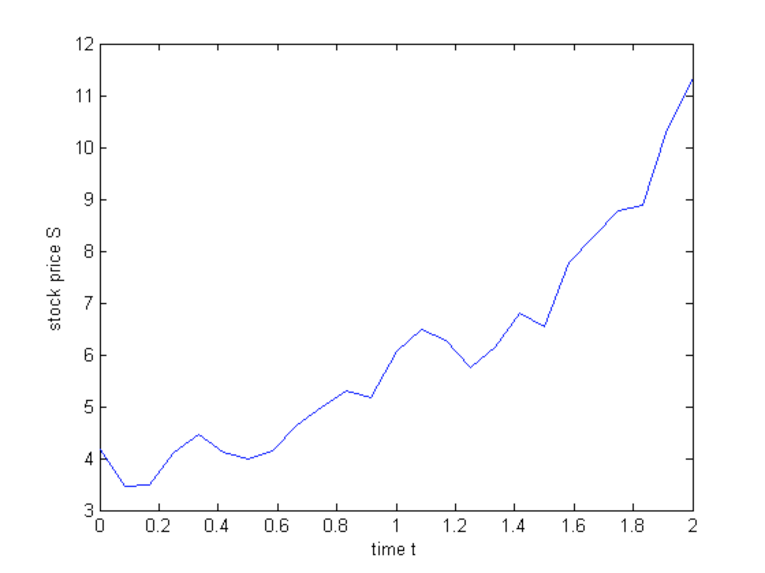
\includegraphics[totalheight=6cm]{pic/tu1}
	\caption{两年的股票走势}
\end{figure}

从图中我们可以看出,合同的价值是一个计息期比计息期要低,在每个实施日前一刻到达本记息期内的最大值,在实施日实施利息后,合同的价值明显的比上一个记息期要低的多,这是因为在给予一定的收益率后,合同的内在价值变小了的原因,虽然每次实施日不一定都能够得到最高的收益率,但是毕竟是少了1次得到收益率的机会了。

